%!TEX root = ../tcc.tex

\chapter{Anatomia do BitTorrent}

O BitTorrent é uma rede \gls{p2p} onde cada um de seus usuários assume o papel híbrido
de servidor, que fornece os arquivos, e de cliente, que adquire os arquivos. Cada
computador é chamado de \gls{peer}.

Cada transferência por BitTorrent está associada a um arquivo de \glspl{metadata}
chamado \gls{torrent}. Esse arquivo contém informações sobre os arquivos que formam o
pacote de dados daquele conjunto de dados e também um ou mais endereços de
\glspl*{tracker}, que mantém listas atualizadas dos \glspl*{peer} que estão
compartilhando os dados, atualizado em períodos de tempo curtos (usualmente 30 minutos).

\begin{comment}
    \begin{figure}[H]
        \centering
        \fbox{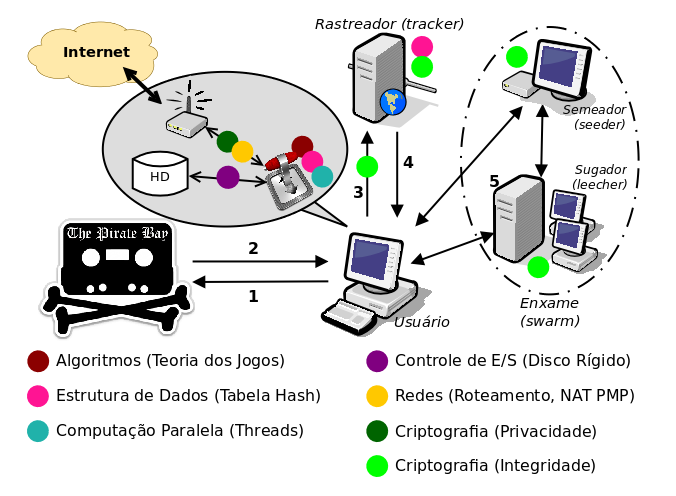
\includegraphics[width=0.64\textwidth]{funcionamento.png}}
        \caption{esquema básico do funcionamento do BitTorrent}
        \label{fig:torrent-basics}
    \end{figure}
\end{comment}

Enquanto um \gls*{peer} estiver fazendo download de um \gls*{torrent} é chamado de
\gls{leecher}, pois ainda estará consumindo dados de outros \glspl*{peer}; quando o
download acabar, passará a ser um \gls{seeder}, que somente envia dados para outros
\glspl*{peer}.

\begin{figure}[ht]
    \centering
    \fbox{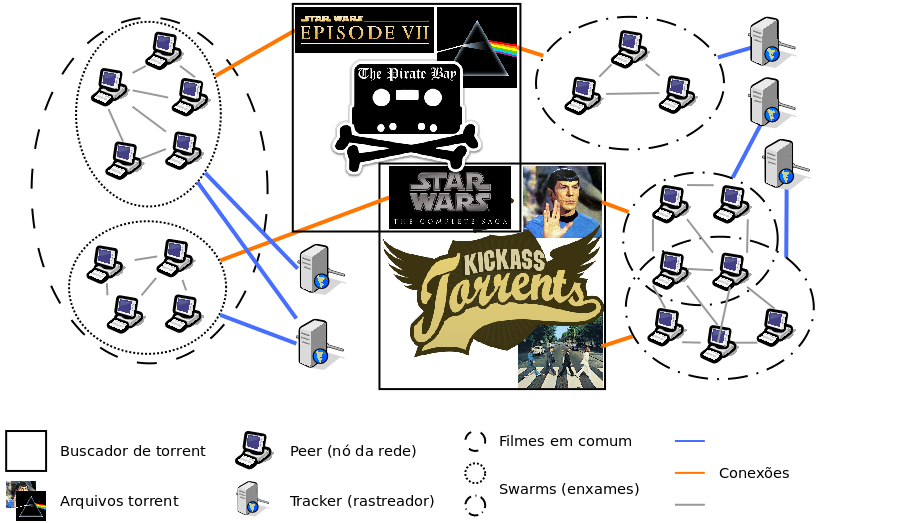
\includegraphics[width=0.85\textwidth]{universobt.png}}
    \caption{amostra de uma rede de conexões BitTorrent}
    \label{fig:torrent-universo}
\end{figure}

Os arquivos \gls*{torrent} ficam disponíveis em vários sites de índice (às vezes
chamados de comunidades), como o \href{http://thepiratebay.sx/}{ThePirateBay}, o
\href{http://kickass.to/}{Kickass} ou \href{https://torrentz.eu/}{Torrentz}, muitas
vezes em mais de um deles ao mesmo tempo. Apesar de todo conteúdo compartilhado possuir
um arquivo \gls*{torrent}, não necessariamente um arquivo \gls*{torrent} está sendo
compartilhado, podendo inclusive estar extinto.

\Glspl*{peer} que participam do compartilhamento de um arquivo \gls*{torrent} específico
fazem parte do \gls{swarm}, onde os dados contidos no pacote desse arquivo são
compartilhados com outros por partes.

\begin{figure}[hp]
    \newlength{\myvsize}
    \newlength{\myhsize}
    \setlength{\myvsize}{5mm}
    \setlength{\myhsize}{0.28\textwidth}

    \centering

    \begin{subfigure}[H]{\myhsize}
        \fbox{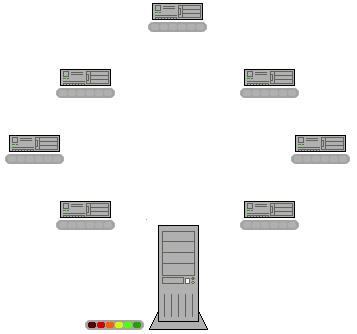
\includegraphics[width=\textwidth]{Torrentcomp_small-0.png}}
        \caption{}
        \label{fig:torrent-repr-0}
    \end{subfigure}%
    \quad %add desired spacing between images (~, \quad, \qquad or blank line)
    \begin{subfigure}[H]{\myhsize}
        \fbox{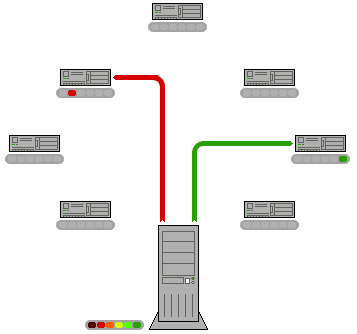
\includegraphics[width=\textwidth]{Torrentcomp_small-1.png}}
        \caption{}
        \label{fig:torrent-repr-1}
    \end{subfigure}%
    \quad
    \begin{subfigure}[H]{\myhsize}
        \fbox{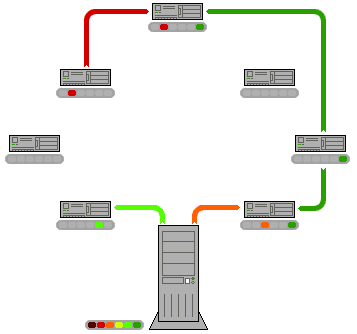
\includegraphics[width=\textwidth]{Torrentcomp_small-2.png}}
        \caption{}
        \label{fig:torrent-repr-2}
    \end{subfigure}

    \vspace{\myvsize}

    \begin{subfigure}[H]{\myhsize}
        \fbox{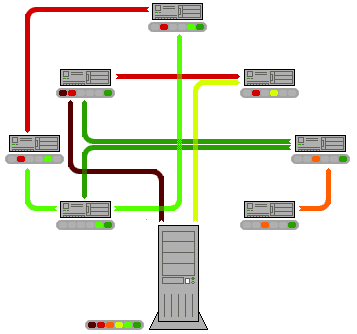
\includegraphics[width=\textwidth]{Torrentcomp_small-3.png}}
        \caption{}
        \label{fig:torrent-repr-3}
    \end{subfigure}%
    \quad
    \begin{subfigure}[H]{\myhsize}
        \fbox{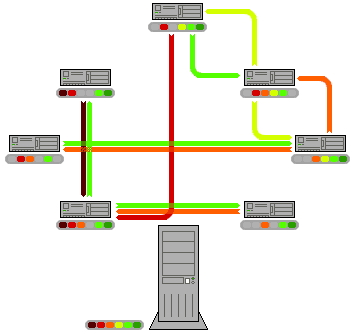
\includegraphics[width=\textwidth]{Torrentcomp_small-4.png}}
        \caption{}
        \label{fig:torrent-repr-4}
    \end{subfigure}%
    \quad
    \begin{subfigure}[H]{\myhsize}
        \fbox{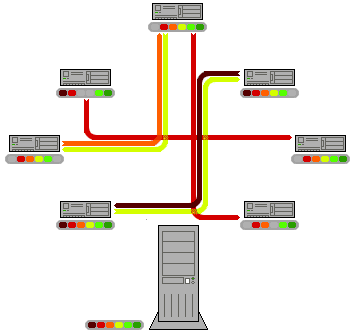
\includegraphics[width=\textwidth]{Torrentcomp_small-5.png}}
        \caption{}
        \label{fig:torrent-repr-5}
    \end{subfigure}

    \vspace{\myvsize}

    \begin{subfigure}[H]{\myhsize}
        \fbox{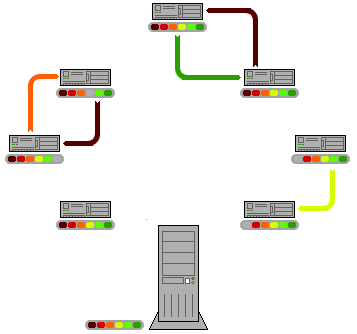
\includegraphics[width=\textwidth]{Torrentcomp_small-6.png}}
        \caption{}
        \label{fig:torrent-repr-6}
    \end{subfigure}%
    \quad
    \begin{subfigure}[H]{\myhsize}
        \fbox{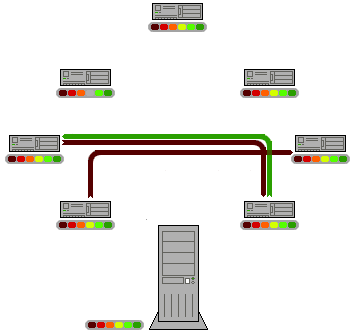
\includegraphics[width=\textwidth]{Torrentcomp_small-7.png}}
        \caption{}
        \label{fig:torrent-repr-7}
    \end{subfigure}%
    \quad
    \begin{subfigure}[H]{\myhsize}
        \fbox{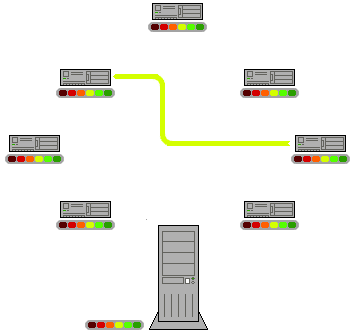
\includegraphics[width=\textwidth]{Torrentcomp_small-8.png}}
        \caption{}
        \label{fig:torrent-repr-8}
    \end{subfigure}

    \vspace{\myvsize}

    \begin{subfigure}[H]{\myhsize}
        \fbox{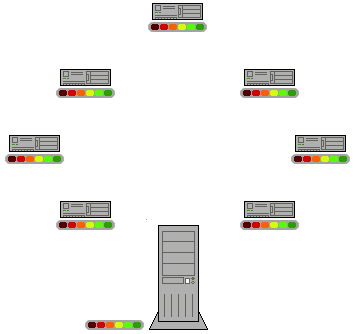
\includegraphics[width=\textwidth]{Torrentcomp_small-9.png}}
        \caption{}
        \label{fig:torrent-repr-9}
    \end{subfigure}

    \caption{Simulação de uma transferência torrent: o \gls{seeder}, na parte
    inferior das figuras, possui todas as 5 partes de um arquivo, que os outros
    computadores, os \glspl{leecher}, baixam de forma independente e paralela. Fonte:
    \cite{fig:torrent-dl}}
    \label{fig:torrent-repr}
\end{figure}

Essas partes variam de acordo com cada arquivo \gls*{torrent}. O tamanho total do
conjunto de arquivos contidos nesse arquivo é dividido em partes de tamanho fixo
(geralmente 256kB) e transmitido de forma independente das outras, seguindo a ordem
estabelecida pelo algoritmo de troca de partes (explicado na seção~\ref{titfortat}),
ordem essa que varia de acordo com o estado atual do \gls*{swarm} para o arquivo
\gls*{torrent} dado.

Todos esses agentes possuem relações de múltiplas entre si. Por exemplo, um mesmo
arquivo \gls*{torrent} pode estar indexado por vários sites indexadores. Como veremos
nos capítulos seguintes, eles contém uma informação que os identificam unicamente entre
si, mantendo a consistência de dados através desses vários sites de busca. Outra
observação a ser feita é que um \gls*{peer} pode estar baixando mais de um
\gls*{torrent} simultaneamente, ou seja, participando de dois \glspl*{swarm} ao mesmo
tempo. Por fim, em alguns casos um arquivo \gls*{torrent} possui grande quantidade de
\glspl*{peer}, havendo necessidade de se dividir o \gls*{swarm} em algumas partes para
fins de escalabilidade da rede formada.

\newpage
\subsection*{Arquivo .torrent}

Ao se adicionar um \gls*{torrent} em um programa cliente, ocorrem muitas transmissões de
dados antes do download de fato. Para demonstrar isso, usaremos um arquivo torrent do
filme ``A Noite dos Mortos Vivos'' de 1960 \cite{torrent-file}, que é de domínio público
e livre de direitos autorais.

Se abrirmos esse arquivo, veremos uma grande \gls{string}, caracteres diferentes e
incomuns, formando um conteúdo ilegível (na seção binária) e sob uma forma compacta,
mostrado no código~\ref{lst:torrent-file-raw}.

\begin{listing}[H]
    \begin{minted}[
        linenos,
        frame=single,
        numbersep=6pt,
        baselinestretch=1,
        fontfamily=courier,
        gobble=4,
        fontsize=\scriptsize
    ]{text}
    d8:announce36:http://bt1.archive.org:6969/announce13:announce-listll36:http://bt1.
    archive.org:6969/announceel36:http://bt2.archive.org:6969/announceee7:comment13:crea
    tiondatei1343715473e4:infod5:filesld5:crc328:030208fe6:lengthi4127671704e3:md532:627
    f5a428f9e454ccfcb29d31b87169a5:mtime10:10794024804:pathl29:night_of_the_living_dead.
    mpege4:sha140:5e44bb1b3f700240249a5287c64dc02dc56d034bee4:name24:night_of_the_living
    _dead12:piecelengthi4194304e6:pieces23720:<binary>

    (...)

    e6:locale2:en5:title24:night_of_the_living_dead8:url-listl28:http://archive.org/
    download/39:http://ia600301.us.archive.org/22/items39:http://ia700301.us.archive.
    org/22/itemsee
    \end{minted}

    \caption{trecho do conteúdo do arquivo .torrent do filme ``A Noite dos Mortos
    Vivos'', de 1960 \cite{torrent-file}, com a parte binária truncada}
    \label{lst:torrent-file-raw}
\end{listing}

Esse conteúdo está organizado usando o formato \gls{bencode}, que é um formato de
codificação compacta de arquivos especial para arquivos \gls*{torrent} e não é legível
ao ser humano. Com alguma formatação, podemos enxergar os componentes separadamente,
como mostra o código~\ref{lst:torrent-file-code}.

Esse conteúdo tem significado, sendo utilizado da seguinte forma
\cite{wikitheory:bencoding}:

\begin{itemize}
    \item \gls*{string} são prefixos de números na base 10 que representam
        comprimentos, seguidos por um caractere `:' e então o conteúdo. Por exemplo, na
        linha 2, \verb|8:announce| corresponde à \gls*{string} "announce".

    \item números são representados por um `i', seguidos do valor na base 10 (sem
        qualquer limite, mas sem zeros precedentes como em $0003$, e podendo ser
        negativo), e terminados por um `e'. Por exemplo, na linha 11,
        \verb|i1343715473e| corresponde ao número 1343715473.

    \item listas são formadas por `l', seguidos por seus elementos (também no formato
        \gls*{bencode}), e então terminados por `e'. Por exemplo, \verb|l3:foo3:bare|
        corresponde a ["foo", "bar"]. No código acima, é presente entre as linhas 43
        e 47.

    \item dicionários são definidos por `d', seguidos de uma lista alternada de chaves e
        seus valores correspondentes, terminando com `e', onde as chaves devem estar
        ordenadas usando-se comparação binária ao invés da usual alfanumérica.
        Por exemplo, a \gls*{string} \verb|d3:foo3:bar6:foobar6:bazbare| corresponde a
        \{"foo: "bar", "foobar": "bazbar"\}, e \verb|d3:fool6:foobar3:bazee| a
        \{"foo": ["foobar", "baz"]\}.
\end{itemize}

\begin{listing}[H]
    \begin{minted}[
        linenos,
        frame=single,
        numbersep=6pt,
        baselinestretch=1,
        fontfamily=courier,
        gobble=4,
        fontsize=\scriptsize
    ]{text}
    d
        8:announce
        36:http://bt1.archive.org:6969/announce
        13:announce-list
        l
            l36:http://bt1.archive.org:6969/announcee
            l36:http://bt2.archive.org:6969/announcee
        e
        7:comment
        13:creation date
        i1343715473e
        4:info
        d
            5:files
            l
                d
                    5:crc32
                    8:030208fe
                    6:length
                    i4127671704e
                    3:md5
                    32:627f5a428f9e454ccfcb29d31b87169a
                    5:mtime
                    10:1079402480
                    4:path
                    l29:night_of_the_living_dead.mpege
                    4:sha1
                    40:5e44bb1b3f700240249a5287c64dc02dc56d034b
                e
            e
            4:name
            24:night_of_the_living_dead
            12:piece length
            i4194304e
            6:pieces
            23720:<binary>
        e
        6:locale
        2:en
        5:title
        24:night_of_the_living_dead
        8:url-list
        l
            28:http://archive.org/download/
            39:http://ia600301.us.archive.org/22/items
            39:http://ia700301.us.archive.org/22/items
        e
    e
    \end{minted}
    \caption{trechos formatados de forma legível do conteúdo do arquivo .torrent do
    filme ``A Noite dos Mortos Vivos'', de 1960 \cite{torrent-file}, com a parte
    binária truncada}
    \label{lst:torrent-file-code}
\end{listing}

\subsection*{Magnet Link}

Além do arquivo \gls*{torrent}, existe uma outra forma de se transmitir os
\glspl*{metadata} necessários para se iniciar a transmissão, que é utilizando
\gls{magnetlink}.

\Glspl*{magnetlink}, ao contrário dos arquivos \gls*{torrent}, não estão gravados em
algum dispositivo de armazenamento. Basicamente, é um esquema de \gls{uri} usado
exclusivamente para o protocolo.

No caso citado, o site de origem do \gls*{torrent} que estamos usando não fornece um
\gls*{magnetlink} oficialmente. Porém, o Transmission consegue construir uma \gls*{uri}
a partir do arquivo original, para fins de compartilhamento direto. O resultado, após
decodificar o endereço para um formato legível (retirando a codificação de caracteres
especiais \cite{wiki:urlencode}) foi o seguinte:

\begin{listing}[ht!]
    \begin{minted}[
        linenos,
        frame=single,
        numbersep=6pt,
        baselinestretch=1,
        fontfamily=courier,
        gobble=4,
        fontsize=\scriptsize
    ]{text}
    magnet:?xt=urn:btih:72d7a3179da3de7a76b98f3782c31843e3f818ee
    &dn=night_of_the_living_dead
    &tr=http://bt1.archive.org:6969/announce&tr=http://bt2.archive.org:6969/announce
    &ws=http://archive.org/download/
    &ws=http://ia600301.us.archive.org/22/items/&ws=http://ia700301.us.archive.org/22/items/
    \end{minted}
    \caption{\gls*{magnetlink} do arquivo .torrent do filme ``A Noite dos Mortos Vivos''
    , de 1960 \cite{torrent-file}, com parâmetros divididos entre linhas para melhor
    visualização}
    \label{lst:torrent-file-magnet-link}
\end{listing}

Esse endereço é composto por vários pares de nomes de parâmetros (sem qualquer ordem
específica) e seus respectivos valores, formando uma \gls{querystring}. Podemos
dividir esse endereço em partes, cada uma tendo o seu significado:

\begin{itemize}
    \item \verb|xt|: parâmetro para \emph{exact topic}, ou tópico exato, contém a
        informação mais importante do \gls*{magnetlink}: o identificador único de
        \gls*{torrent}. Serve para encontrar e verificar os arquivos especificados.
        No caso, \verb|urn:btih:<hash>| corresponde ao \gls{urn} \verb|btih|
        (\emph{BitTorrent Info Hash}), que é a \gls*{string} \gls{hashvalue} resultado
        da \gls{hashfunction} SHA-1, convertida para hexadecimal

    \item \verb|dn|: parâmetro que contém o \emph{display name}, ou nome de
        visualização, contém um nome que é mostrado para o usuário, por conveniência

    \item \verb|tr|: o \emph{address tracker}, ou endereço do \gls*{tracker}, onde o
        programa cliente vai procurar as informações de \glspl*{peer}

    \item \verb|ws|: endereço do arquivo para \emph{webseed}, ou fornecimento web,
        que é o endereço do arquivo em um servidor HTTP ou FTP, sendo utilizado como
        alternativa a um \gls*{swarm} problemático \cite{wiki:torrent}
\end{itemize}

\section{Busca por informações}

Para cada \gls*{swarm} gerenciado, o \gls*{tracker} possui uma lista dos \glspl*{peer}
que participam dele, que é enviada ao \gls*{peer} que a quer, quando este faz um pedido
por meio de uma requisição \gls{httpget}. Quando essa requisição é recebida pelo
\gls*{tracker}, este inclui ou atualiza o registro do \gls*{peer} solicitante e devolve
para ele uma lista de 50 \glspl*{peer} aleatórios, de forma uniforme, que fazem parte do
\gls*{swarm}. Não havendo essa quantidade total, a lista toda é enviada ao requisitante;
caso contrário, a aleatoriedade proporciona uma diversidade de listas enviadas,
proporcionando robustez ao sistema \cite{wikitheory:tracker-response}.

Esse contato de um \gls*{peer} com o \gls*{tracker} é chamado de \gls{announce}, e
ocorre nas seguintes situações:

\begin{itemize}
    \item no primeiro contato do \gls*{peer}, para que ele tenha acesso a um
        \gls*{swarm}

    \item a cada período de tempo, estipulado pelo tracker, para que o \gls*{peer}
        continue mostrando que ainda está conectado, além de pode receber endereços de
        \glspl*{peer} novos

    \item quando a quantidade de \glspl*{peer} conhecidos que estão ativos é menor do 5

    \item quando terminar o download, notificando que passou a ser um \gls*{seeder}

    \item quando sai do \gls*{swarm}, seja por desconexão ou por encerramento do
        programa cliente
\end{itemize}

Além do \gls*{announce}, outra forma de troca de informação entre \glspl*{peer} e
\glspl*{tracker} é pelo \emph{scrape}. Geralmente usado pelos programas cliente para
decidir quando realizar um \gls*{announce}, informa o número de \glspl*{peer},
\glspl*{leecher} e \glspl*{seeder} de uma lista de um ou mais \glspl*{torrent}. É dessa
forma que os sites de indexação sabem dessas informações e as apresentam nas páginas.

No \gls*{announce}, vários dados devem ser enviados ao \gls*{tracker}. São eles:

\begin{itemize}
    \item \textbf{info\_hash}: \gls*{hashvalue} de 20 bytes resultante da
    \gls*{hashfunction} SHA-1 com \gls*{urlencode} do valor da chave \verb|info| do
    arquivo de \gls*{metadata}

    \item \textbf{peer\_id}: \gls*{string} com \gls*{urlencode} de 20 bytes usado como
    identificador único do programa cliente, gerado no ínício da sua execução. Para
    isso, provavelmente deve incorporar informações do computador, a fim de se gerar um
    valor único para o computador

    \item \textbf{uploaded}: a quantidade total de dados, em bytes, enviados desde
    quando o cliente enviou o primeiro aviso ao \gls*{tracker}

    \item \textbf{downloaded}: a quantidade total de dados, em bytes, recebidos desde
    quando o cliente enviou o primeiro aviso ao \gls*{tracker}

    \item \textbf{left}: a quantidade total de dados, em bytes, que faltam para o
    requisitante terminar o download do \gls*{torrent} e passe a ser um \gls*{seeder}

    \item \textbf{compact} (opcional): se o valor passado for 1, significa que o
    requisitante aceita respostas compactas. A lista de \glspl*{peer} enviada é
    substituída por uma \gls*{string} de peers, cada um com 6 bytes, onde os 4 bytes
    iniciais são o host e os 2 bytes finais são a porta de transmissão. Por exemplo, o
    endereço IP 10.10.10.5:80 seria transmitido como \verb|0A 0A 0A 05 00 80|. Deve-se
    observar que alguns \glspl*{tracker} suportam somente conexões deste tipo para
    otimização da utilização da banda de rede e, pra isso, ou recusam requisições sem
    \verb|compact=1| ou, caso não as recusem, enviam respostas compactas a menos que a
    requisição possua \verb|compact=0|

    \item \textbf{no\_peer\_id} (opcional): sinaliza que o \gls*{tracker} por omitir o
    campo ``\gls*{peer} id'' no dicionário de \glspl*{peer}. É ignorado caso o modo
    compacto esteja habilitado

    \item \textbf{event} (opcional): pode possuir os valores ``started'' (iniciado),
    ``completed'' (terminado), ``stopped'' (parado), ou vazio para não especificar.
    \begin{itemize}
        \item started : a primeira requisição para o \gls*{tracker} deve enviar este
        valor
        \item stopped : avisa que o programa cliente está fechando
        \item completed : quando o download que estava ocorrendo termina, ou seja, não
        é enviado quando o programa cliente inicia com o \gls*{torrent} em 100\%
    \end{itemize}

    \item \textbf{port} (opcional): o número da porta de conexão que o programa cliente
    está escutando por transmissões de dados. Em geral, portas reservadas para
    BitTorrent estão entre a 6881 e a 6889. Se esse for o caso, pode ser omitido

    \item \textbf{ip} (opcional): o endereço IP verdadeiro do requisitante no formato
    legível do IPv4 (4 conjuntos de número de 0 a 255 separados por `.') ou do IPv6 (8
    conjuntos de números hexadecimais de 4 dígitos separados por `:'). Não é sempre
    necessário, pois o endereço pode ser conhecido através da requisição. Assim, é usado
    quando o programa cliente está se comunicando com o \gls*{tracker} através de um
    \gls{proxy} ou quando ambos cliente e \gls*{tracker} estão no mesmo lado local de um
    \gls{nat}, pois nesse caso o endereço IP não é roteável

    \item \textbf{numwant} (opcional): quantidade de \glspl*{peer} que o requisitante gostaria de receber do \gls*{tracker}. É permitido valor zero. Se omitido, assume valor padrão de 50

    \item \textbf{key} (opcional): mecanismo de idetificação adicional para o programa cliente provar sua identidade caso tenha ocorrido mudança no seu endereço IP

    \item \textbf{trackerid} (opcional): se a resposta de um \gls*{announce} anterior
    continha o endereço IP de um \gls*{tracker}, deve ser enviado neste campo
\end{itemize}

\todo[inline]{explicar como o Transmission usa o torrent}

\section{Fontes de arquivos}

Mostrarei o processamento dos dados adquiridos na seção anterior e como ele organiza a lista das fontes de arquivos usando a tabela hash DHT Kademlia.

\section{Jogo da troca de arquivos}

Explicarei o algoritmo tit-for-tat padrão do protocolo BitTorrent, que vem da Teoria dos Jogos, e como o Transmission o implementa.

\afterpage{\clearpage}